Given the size of the data our software will be working on, it requires an efficient way of storing them.

There are 2 kinds of data, on the first hand the ones the programs works on; on the other hand, the parameters and utilities.
\subsection{Boards and nodes}
Boards are stored as bitboard. As the game is played on a 8x8 board, it is convinient to use a 64 bit integer to store the positions of the pieces. That way, each and every of a kind of pieces are stored on the same integer, saving space compared to a matrix 8 x 8. Players own rabits, cats, dogs, horses, camel and elephant; thus using 6 integer for each player do the job. Adding an additionnal bitboard to store the position of every pieces of each players helps to increase the speed of the algorithm by reducing the number of test required to be done during the playout phases.

\begin{figure}[H] 
\centerline{\includegraphics[scale=0.8]{Data_Structure/Img/Node.png}}
\caption{\label{fig:array}\textit{Details of the data cointained in a node}.}
\end{figure}
Nodes contains statistics about the previous results, a pointer to their parent, a pointer to the first of their children and the number of children they own. They are stored in an array set at the begining of the program, thus grouping them on a countinuous memory segment. Therefore the time to gain access to them is decreased.
\begin{figure}[H] 
\centerline{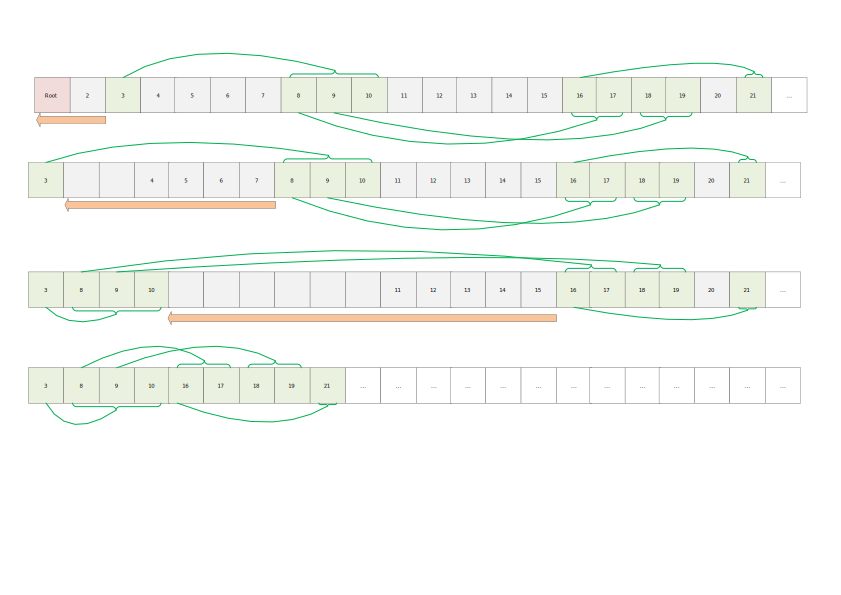
\includegraphics[width=\textwidth]{Data_Structure/Img/array.png}}
\caption{\label{fig:array}\textit{Prunning of the tree}.}
\end{figure}
In order to prune the tree, we use the following method : create a copy of the current tree (\textit{\_tree}) into a buffer (\textit{\_buff}). The root of the buffer tree will be a copy the chosen node. Then the children are saved going up through the branches. The advantage of this method is that you only copy the nodes you want to keep. However the memory used of the buffer need to be the same as the one of the tree before the prunning. Thus the maximum memory that can be used by the tree (\textit{\_tree}) is half the memory used by the program. In order to dermine the number of leaves to be created, the program check how much memory there is left on the computer and use a fixed percentage of it.
\begin{equation}
N = \frac{R \times 90\%}{2}
\end{equation}
\ensuremath{N} = number of leaves.\\
\ensuremath{R} = RAM left to use.

We chose to limit the memory used by the tree to 90\% of the aviable memory in order to not overload the RAM and to let some left for other operations such as simulations.
\subsection{Utilities and parameters}
